\documentclass[11pt]{amsart}
%\documentclass[11pt]{report}
\usepackage[toc,page]{appendix}
\usepackage{float}
\usepackage{mathtools}
\usepackage{geometry}        % See geometry.pdf to learn the layout options.
\geometry{a4paper}           % ... or a4paper or a5paper or ...
%\geometry{landscape}        % Activate for for rotated page geometry
%\usepackage[parfill]{parskip} % Activate to begin paragraphs with empty line
\usepackage{graphicx}
\usepackage{amssymb}
\usepackage{epstopdf}

\usepackage[most]{tcolorbox}
\definecolor{block-gray}{gray}{0.85}
\newtcolorbox{myquote}{colback=block-gray,grow to right by=+0mm,grow to left by=-10mm, boxrule=0pt,boxsep=0pt,breakable}

\DeclareGraphicsRule{.tif}{png}{.png}{`convert #1 `dirname #1`/`basename #1 .tif`.png}
\graphicspath{ {images/} }

\renewcommand{\familydefault}{\sfdefault}
\newcounter{defctr}

\title{Naigama parsing system (Compendium)}
\author{Kees-Jan Hermans}
%\date{}                     % Activate to display a given date or no date

\begin{document}
\maketitle

This document contains a description of Naigama, a software
implementation of a Parsing Expression Grammar compiler,
assembler, and bytecode execution engine.

\vspace*{3\baselineskip}

\begin{figure}[H]
\centering
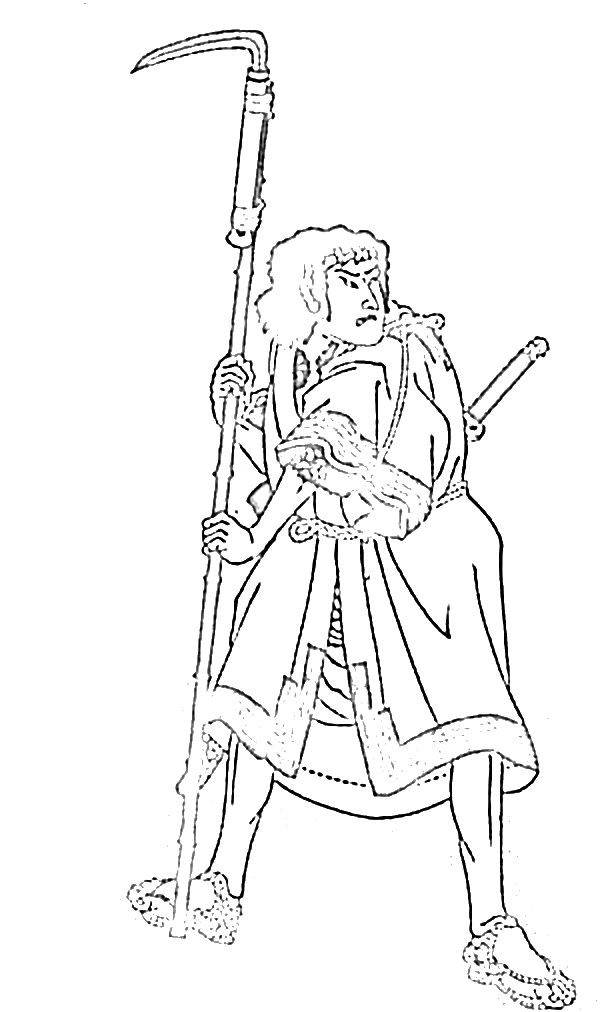
\includegraphics[width=60mm]{naigama}
\end{figure}

\vfill

\begin{table}[]
\centering
\begin{tabular}{ll}
Accompanies release & \input{../release} \\
Author &  Kees-Jan Hermans / kees.jan.hermans@gmail.com \\
Classification & - \\
Generated on & \today \\
\end{tabular}
\end{table}

% Accompanies release: \input{../../release}
% 
% Author: Kees-Jan Hermans / kees.jan.hermans@gmail.com
% 
% Classification: -
% 
% Generated on: \today
\newpage

\tableofcontents

\setlength{\parindent}{4em}
\setlength{\parskip}{1em}

\newpage
\section{Overview}

This document describes the Naigama parsing system, which is a 
modular system to process structured arbitrary length data inputs,
in order to extract meaning from it (matching, capturing), or to
manipulate it (replacements).
The system was designed with a focus on information and system security.

The system comes in three parts: a grammar compiler, an assembler,
and a bytecode execution engine. Each of the parts has their own
input file format specification (grammar description, assembly specification,
and bytecode specification). The process in brief: the compiler takes a
grammar description that the human end user has made, and turns it into
an assembly language. The assembler takes the assembly, and turns it
into a bytecode. The engine takes the bytecode and the input, and
processes it, resulting either in (various measures of) failure or
success.

The reason for this modularity is strict separation of tasks, and openness:
anyone should be able to take out a module, and replace it with one
of their own.
It should be expressly possible to take out the compiler, and replace
it with another tool that produces the Naigama assembly, for example.
Or have a different engine. Or write an optimizer for the assembly.

\subsection{On Grammar}
  
Naigama grammar is the human interface of the system.
It can be used to define complex syntax definitions in order
to match, capture from, and replace in, structured inputs.

People familiar with regular expressions \cite{bib:regex},
Backus-Naur syntax descriptions \cite{bib:backusnaur},
and / or Lex and Yacc tools \cite{bib:yacc},
should find this part of the document relatively easy to understand.
The ideas underlying Naigama grammar, assembly and bytecode
are heavily borrowed from Lua PEG (LPEG) \cite{bib:peg}
by Roberto Ierusalimschy et al.

\subsection{On Assembly}

The Naigama assembly language is a mixture of two languages:
For one, it is the outcome instruction set, according to the
aforementioned LPEG whitepaper,
of the Naigama grammar compilation process. However, it also contains
instructions that won't be produced by this compiler, but may
either be produced by a separate optimizer, or other compilers
altogether (for example, one that focuses on network packet
parsing).

The Naigama assembly language, in all cases, is the human readable
variant of the Naigama bytecode, and its instructions are one-on-one
translatable from the one to the other, and vice versa
(although labels will be lost in the reverse process).

\subsection{On Bytecode}

Naigama bytecode is the machine interface of the system.
It runs in the Naigama engine against the input provided by the user.
It is designed to be:

\begin{itemize}

\item Easy and quick to interpret.
\item Resilient against bit upset events.
\item Resilient against endless loops.
\item Usable while keeping both bytecode and input as read-only buffers.

\end{itemize}


\newpage
\section{Grammar}
\label{sec:grammar}

A Naigama grammar file or buffer consists either of a single
unnamed expression, or of a sequence of named expressions (called rules),
whitespace and comments, denoted in ASCII text.
Naigama grammar is defined with the express purpose of matching, validating
and/or capturing from an arbitrary data input.
Naigama grammar is taken by the Naigama compiler program (naic) and turned
into Naigama assembly [section \ref{sec:assembly}].

\begin{myquote}
\begin{verbatim}
-- JSON; JavaScript Object Notation.

TOP          <- JSON
__prefix     <- %s*
JSON         <- HASH END
HASH         <- CBOPEN OPTHASHELTS CBCLOSE
OPTHASHELTS  <- HASHELTS / ...
HASHELTS     <- HASHELT COMMA HASHELTS / HASHELT
HASHELT      <- STRING COLON VALUE
ARRAY        <- ABOPEN OPTARRAYELTS ABCLOSE
OPTARRAYELTS <- ARRAYELTS / ...
ARRAYELTS    <- VALUE COMMA ARRAYELTS / VALUE
VALUE        <- STRING / FLOAT / INT / BOOL / NULL / HASH / ARRAY
STRING       <- { '"' ( '\\' ([nrtv"] / [0-9]^3) / [^"\\] )* '"' }
INT          <- { [0-9]+ }
FLOAT        <- { [0-9]* '.' [0-9]+ }
BOOL         <- { 'true' / 'false' }
NULL         <- { 'null' }
CBOPEN       <- '{'
CBCLOSE      <- '}'
ABOPEN       <- '['
ABCLOSE      <- ']'
COMMA        <- ','
COLON        <- ':'
END          <- !.

\end{verbatim}
\end{myquote}
\textit{Example of a Naigama grammar meant to validate and capture from
JSON\cite{bib:json} text.}

\subsection{Rules}

A rule is defined as an \textit{Identifier}, followed by a
left-pointing arrow (composed of a less-than and a minus sign),
followed by a matching expression.

When a Naigama grammar consists of a sequence of rules
(as opposed to a single line expression),
the first rule is used as the starting point for matching inputs.

\begin{myquote}
\begin{verbatim}
RULE1 <- 'a' / RULE2
RULE2 <- 'b' / RULE3
RULE3 <- 'c'

\end{verbatim}
\end{myquote}
\textit{Definition of a set of rules}

\subsubsection{Identifiers}

Identifiers, in Naigama, are defined as a combination of letters,
numbers and the underscore character, not starting with a number,
of between one and 64 characters long.

\begin{myquote}
\begin{verbatim}
IDENTIFIER <- [a-zA-Z_][a-zA-Z0-9_]^-63

\end{verbatim}
\end{myquote}
\textit{Definition of an identifier}

Identifiers are used to start rule definitions, and as references
to rules in expressions.

\subsubsection{Special Rules}

There is currently one special rule in Naigama grammar: a rule called
'\_\_prefix' will be treated specially. This rule will be, from its
definition onwards, called before the execution of any subsequent rule
definition expression. The aim is to make whitespace and comment filtering
in program language parsing easier. See also the earlier 'JSON' grammar
example.

\subsection{Expressions}

Expressions are lists of terms, optionally separated by the
OR operator (denoted by the forward slash sign).

\subsection{Terms}

\subsection{Matchers}

\subsubsection{NOT and AND Modifiers}

\subsubsection{Quantifiers}

\subsubsection{The ANY Matcher}

The ANY matcher also allows you to define end-of-input, like so:

\begin{myquote}
\begin{verbatim}
ENDOFINPUT <- !.

\end{verbatim}
\end{myquote}
\textit{Definition of end-of-input}

\subsubsection{The SET Matcher}

\subsubsection{The STRING Matcher}

\subsubsection{The BITMASK Matcher}

\subsubsection{The HEXLITERAL Matcher}

\subsubsection{The VARCAPTURE Matcher}

\subsubsection{The CAPTURE Matcher}

\subsubsection{The GROUP Matcher}

\subsubsection{The MACRO Matcher}

\subsubsection{The VARREFERENCE Matcher}

\subsubsection{The REFERENCE Matcher}




\newpage
\section{Assembly}
\label{sec:assembly}

A Naigama assembly file or buffer consists of sequences of
whitespace, comments, labels, and (parametrized) instructions, separated
by new lines, and denoted in ASCII text.

Naigama assembly is taken by the Naigama assembler program (naia) and turned
into bytecode.

\begin{myquote}
\begin{verbatim}
-- Compilation of: TEST <- { 'a' } { 'a' } { 'a' / 'b' }

  call TEST
  end
-- Rule
TEST:
  opencapture 0
  char 61
  closecapture 0 0
  opencapture 1
  char 61
  closecapture 1 0
  opencapture 2
  catch __LABEL_30 -- alternative
  char 61
  commit __LABEL_31
__LABEL_30:
  char 62
__LABEL_31:
  closecapture 2 0
  ret

\end{verbatim}
\end{myquote}
\textit{Example of a piece of Naigama assembly}

\subsection{Comments}

Just like in Naigama grammar,
comments in Naigama assembly start with two minus signs, and end at
a new line. They can be given on separate lines, or they can be
postfixed to instructions or labels.

\subsection{Labels}

Labels are identifiers (the same identifiers as in their definition
in the grammar chapter) or numbers, followed by a colon sign. They are used
as positions for the bytecode to jump to, when used by instructions.

When performing the assembly, the Naigama assembler program resolves
each label to their offset in the resultant bytecode, and replaces each
reference to a label with that offset.

Labels don't quite disappear though - you have the option to make the
assembler program emit a so called 'labelmap' file, which stores the old
label names, mapped to the bytecode offsets given by the assembler,
and which can be used later
for debugging purposes by the bytecode execution engine.

When disassembling (bytecode to assembly), each instruction is always
prefixed by a label in the form of the instruction's offset in decimal,
so that jumps are always correct (but non descriptive).

\subsection{Instructions}


%\begin{table}[]
\begin{center}
\caption{Naigama Assembly Instructions}
\label{tab:naig_assembly}
\begin{longtable}{lll}
\textbf{Mnemonic} & \textbf{Param1} & \textbf{Param2} \\
\endhead
'any' &  &  \\
'backcommit' &  & LABEL \\
'call' &  & LABEL \\
'catch' &  & LABEL \\
'char' & char &  \\
'closecapture' & slot &  \\
'commit' &  & LABEL \\
'condjump' & register & LABEL \\
'counter' & register & value \\
'end' & code &  \\
'endisolate' &  &  \\
'endreplace' &  &  \\
'fail' &  &  \\
'failtwice' &  &  \\
'intrpcapture' &  &  \\
'isolate' & slot &  \\
'jump' &  & LABEL \\
'maskedchar' & char & mask \\
'noop' &  &  \\
'opencapture' & slot &  \\
'partialcommit' &  & LABEL \\
'quad' & quad &  \\
'range' & from & until \\
'replace' & slot & LABEL \\
'ret' &  &  \\
'set' & set &  \\
'skip' & number &  \\
'span' & set &  \\
'testany' &  & LABEL \\
'testchar' & char & LABEL \\
'testquad' & quad & LABEL \\
'testset' & set & LABEL \\
'trap' &  &  \\
'var' & slot &  \\
\end{longtable}
\end{center}
%\end{table}


See table [\ref{tab:naig_assembly}].

\subsection{Parameters}

Parameters follow the instruction in assembly text. They are separated
from the instruction and any other parameters by spaces. The following
types of parameters exist:

\subsubsection{Characters}

Character parameters are denoted as two byte hexadecimal values.

\subsubsection{Quads}

Quad parameters are denoted as eight byte hexadecimal values.

\subsubsection{Sets}

Set parameters are denoted as 64 byte hexadecimal values, representing
a bitmask of 256 possible booleans.

\subsubsection{Registers, Slots, Codes and Numbers}

These parameters are all denoted as decimal numbers.


\newpage
\section{Bytecode}
\label{sec:bytecode}


%\begin{table}[]
\begin{center}
\caption{Naigama Bytecode Instructions}
\label{tab:naig_bytecode}
\begin{longtable}{lllll}
\textbf{Mnemonic} & \textbf{Opcode} & \textbf{Param1} & \textbf{Param2} & \textbf{Length} \\
\endhead
any & 000003e4 &  &   & 4 \\
backcommit & 000403c0 & address &   & 8 \\
call & 00040382 & address &   & 8 \\
catch & 00040393 & address &   & 8 \\
char & 000403d7 & char &   & 8 \\
closecapture & 00040300 & slot &   & 8 \\
commit & 00040336 & address &   & 8 \\
condjump & 00080321 & register & address  & 12 \\
counter & 00080356 & register & value  & 12 \\
end & 000400d8 & code &   & 8 \\
endisolate & 00003005 &  &   & 4 \\
endreplace & 00000399 &  &   & 4 \\
fail & 0000034b &  &   & 4 \\
failtwice & 00000390 &  &   & 4 \\
intrpcapture & 0008000f &  &   & 12 \\
isolate & 00043003 & slot &   & 8 \\
jump & 00040333 & address &   & 8 \\
maskedchar & 00080365 & char & mask  & 12 \\
mode & 0004000a &  &   & 8 \\
noop & 00000000 &  &   & 4 \\
opencapture & 0004039c & slot &   & 8 \\
partialcommit & 000403b4 & address &   & 8 \\
quad & 0004037e & quad &   & 8 \\
range & 000803bd & from & until  & 12 \\
replace & 00080348 & slot & address  & 12 \\
ret & 000003a0 &  &   & 4 \\
scr\_add & 0000050c &  &   & 4 \\
scr\_array & 00040006 &  &   & 8 \\
scr\_assign & 000005c9 &  &   & 4 \\
scr\_bitand & 00000527 &  &   & 4 \\
scr\_bitnot & 00000574 &  &   & 4 \\
scr\_bitor & 0000053c &  &   & 4 \\
scr\_bitxor & 0000052d &  &   & 4 \\
scr\_builtin & 000407cf &  &   & 8 \\
scr\_call & 00040503 &  &   & 8 \\
scr\_condjump & 0004000c &  &   & 8 \\
scr\_dec & 0000053a &  &   & 4 \\
scr\_div & 00000581 &  &   & 4 \\
scr\_equals & 0000056c &  &   & 4 \\
scr\_gt & 0000056f &  &   & 4 \\
scr\_gteq & 0000054d &  &   & 4 \\
scr\_inc & 000005f6 &  &   & 4 \\
scr\_index & 00000009 &  &   & 4 \\
scr\_logand & 0000052e &  &   & 4 \\
scr\_lognot & 000005f9 &  &   & 4 \\
scr\_logor & 000005a9 &  &   & 4 \\
scr\_lt & 00000595 &  &   & 4 \\
scr\_lteq & 00000522 &  &   & 4 \\
scr\_mul & 0000058b &  &   & 4 \\
scr\_nequals & 00000572 &  &   & 4 \\
scr\_pop & 000005cc &  &   & 4 \\
scr\_pow & 00000542 &  &   & 4 \\
scr\_push & 000c0003 &  &   & 16 \\
scr\_ret & 00000555 &  &   & 4 \\
scr\_shift & 00040005 &  &   & 8 \\
scr\_shiftin & 0000057d &  &   & 4 \\
scr\_shiftout & 00000517 &  &   & 4 \\
scr\_string & 000017bb &  &   & 4 \\
scr\_sub & 000005bb &  &   & 4 \\
set & 002003ca & set &   & 36 \\
skip & 00040330 & number &   & 8 \\
span & 002003e1 & set &   & 36 \\
testany & 00040306 & address &   & 8 \\
testchar & 0008039a & address & char  & 12 \\
testquad & 000803db & address & quad  & 12 \\
testset & 00240363 & address & set  & 40 \\
trap & ff00ffff &  &   & 4 \\
var & 000403ee & slot &   & 8 \\
\end{longtable}
\end{center}
%\end{table}


\subsection{Bytecode Structure}

A Naigama bytecode file or buffer consists of a sequence of binary
instructions which, in turn, each consist of a binary
encoded opcode, plus their parameters, should they have any.

The amount and kind of parameters following an opcode, is strictly
defined:
the same opcode will always be followed by the same kinds of parameters
and therefore, an instruction type will always be the same size
(see table [\ref{tab:naig_bytecode}]).

Naigama bytecode is taken by the Naigama engine program (naie) or
library, and run against an input, to produce an output.

\subsection{Opcode Values}

Opcode values are determined through

\begin{itemize}
\item Grouping; 
\item Hamming distance;
\item Instruction size;
\end{itemize}

\subsection{Noop Slides and Canaries}

Implementations that want each instruction to have exactly the
same size, can choose to pad the encoding of shorter instructions
with either no-ops, or canaries.

\subsection{Encoding of Parameters}

\subsubsection{Address}

\subsubsection{Char}

\subsubsection{Slot}

\subsubsection{Register}


\newpage
\section{Engine}
\label{sec:engine}

The Naigama bytecode execution engine or library can be used to
match or fail an input of data using a bytecode.
Both bytecode and input are defined as a buffer of memory with
a certain length. The bytecode buffer may be the result of
the Naigama assembly process; the input is arbitrary data.

\subsection{Order of Execution}

Execution will start with the engine setting the current bytecode
offset to zero.

The engine will execute the instruction at the current bytecode
offset, and then either jump
to another offset within the bytecode if this is the result of
the instruction execution, or to the next instruction, which is
located at the current bytecode offset, plus the size of the
instruction. Bear in mind that instructions have different sizes;
the size of the instruction is a function of the opcode.
This is specified in table [\ref{tab:naig_bytecode}].

Execution ends when an abnormal state is encountered, the FAIL
condition extinguishes the entire stack, or the 'end' instruction
is encountered.

\subsection{Execution States}

The engine must at least provision the following state during execution
of the bytecode buffer.

\subsubsection{Bytecode Offset}

The bytecode offset is an offset in the bytecode. Its value is
between zero (inclusive) and the length of the bytecode (exclusive)
minus four, and is always a multiple of four.

\subsubsection{Input Position}

The input position is the position in the input buffer. Its value
is between zero (inclusive) and the length of the input buffer (exclusive).

\subsubsection{Stack}

The stack is a Last-in-first-out list of items. There are two types
of items that can be on the stack, and there are two instructions that
push each of these items:

\begin{itemize}

\item A 'call' instruction makes the engine jump to a certain address,
but it also pushes a return address on the stack
(this is the address of the instruction following the 'call' instruction),
so that when a 'ret' instruction is encountered,
and this item is popped from the stack, the engine knows where to continue.

Alternatively, a FAIL condition may pop these items from the stack as well.

\item A 'catch' instruction pushes an item on the stack which saves the
engine's state at that point, and contains an alternative address to jump
to. The engine's state is represented by the bytecode offset, the input
position, and the length of the action list.

These items are removed by their corresponding 'commit' instructions however,
a FAIL condition in this case pops the stack item, but then restores the
engine's state and jumps to the alternative address.

\end{itemize}

\subsubsection{Action List}

The action list contains actions related to capturing from the input buffer.
It may contain the following type items:

\begin{itemize}

\item A 'opencapture' type element, which contains an input position
      and a slot number.
\item A 'closecapture' type element, which contains an input position
      and a slot number.
\item A 'replace' type element, which contains two offsets.

\end{itemize}

\subsubsection{Register}

\subsection{Special Conditions}

\subsubsection{Running out of Stack or Actions}

Naigama parsing is a left recursing, meaning that the following
expression:

\begin{myquote}
\begin{verbatim}
INPUT <- ( { . } INPUT ) / ( { . } !. )

\end{verbatim}
\end{myquote}

will be compiled to bytecode that will incur, during its execution,
a stack that is as long as its input, and after execution, will result
in an action list that is as long as the input. Given that Naigama
allows you to process ('arbitrarily') large inputs, this may not
be something that the memory limits of your engine can handle.

When the engine encounters limits on its room for stack or action
list elements, it must hald execution of the bytecode abnormally.

\subsubsection{Streaming Input}

Given that each FAIL cleans up the stack completely until the first
'catch' element, input offsets before the input offset mentioned in the
engine's saved state in the first stack 'catch' item (seen from the top,
if it's given that stacks grown down), can be discarded by the engine,
allowing a streaming model of input provisioning.

\subsubsection{Endless Loops}

Endless loop detection, for a Naigama bytecode execution engine, is
relatively easy: the second time the same combination of bytecode offset
and input position is encountered, an endless loop is occurring, and the
engine should halt execution of the bytecode abnormally.

\subsubsection{Faulty Bytecode / Canary Traps}

Bytecode instruction values have been chosen in such a manner, that the
Hamming distance between them is always two or more, meaning that it
requires more than two bit upset events in an instruction, to potentially
be confused with another.

Addresses are always a multiple of four, so the two least relevant bits
on an address must always be zero.

Compilers may introduce noops or traps in regions that they know should
not ever be jumped to, for example by surrounding good code with them;
the assembly languages expressly allows for this (the 'trap' instruction).

\subsection{Output States}

The engine may exit for the following (negative) reasons:

\begin{itemize}

\item Because a FAIL condition ate up the entire stack, indicating
the the input did not match the compiled pattern or rules.
This is desired behavior.

\item Because the bytecode was correct, but behaved unacceptably
(\textit{ie} room on the stack ran out, or an endless loop was detected).
This is undesirable behavior; better bytecode must be produced
or better engine tuning must be done.

\item Because the bytecode had errors in it
(faulty instruction, faulty offset). This is undesirable behavior;
the bytecode must be re-generated, or a bit upset event must be assumed.

\end{itemize}

And it may be used, when successful, in the following ways:

\begin{itemize}

\item An 'end' instruction was encountered (there was a match).

\item An 'end' instruction was encountered, including an end code
(when a pattern yields several success end points).

\item The action list can be used, read-only on the input (captures).

\item The action list can be used, read-write on the input
(captures / replacements).

\end{itemize}

\subsection{Execution}

When the engine runs bytecode, it will start with the instruction
at bytecode offset zero. It will read and execute this instruction
and run each subsequent instruction (either because it was jumped to
or because it was logically the next instruction).
This loop will continue either until the stack is made empty by a FAIL
condition, or an 'end' instruction is encountered
(or any of the abnormal conditions as noted above were encountered).

The following permutations of the engine's state exist during this loop:

\subsubsection{FAIL}

The FAIL condition is invoked automatically when instructions
that implement input matching, fail, but it may also be invoked
expressly by the 'fail' and 'failtwice' instructions.

A FAIL condition starts eating up the stack, until it encounters
a 'catch' element. When that happens, the 'catch' element is popped,
the state of the engine captured therein is restored, and the engine
jumps to the offset encapsulated therein.

When no 'catch' element is encountered on its way to the top of the stack,
the execution ultimately ends with failure.

\subsubsection{Instruction: Any}

The any instruction checks to see if there is a byte left in the input
and if so, consumes it (by jumping one position forward in the input),
and goes on to the next instruction.

If there is no byte left in the input, then a FAIL is invoked.

\subsubsection{Instruction: Backcommit}

The backcommit instruction eats up the stack like FAIL does,
reconstituting the state captured in the popped, topmost 'catch' element,
but instead of jumping to the offset captured therein, it jumps to
a given parameter offset.

\subsubsection{Instruction: Call}

The call instruction pushes a 'call' element on the stack, which contains
a bytecode offset to continue from (the next instruction), once the
corresponding 'ret' instruction pops this element off the stack.

\subsubsection{Instruction: Catch}

The catch instruction pushes a 'catch' element on the stack, capturing
the current state, and a bytecode offset to jump to, when the FAIL
condition pops this element.

\subsubsection{Instruction: Char}

The char instruction checks to see if there is a byte left in the input
and if so and if it compares to the given parameter character value, 
consumes it (by jumping one position forward in the input),
and goes on to the next instruction.

If there is no byte left in the input, then a FAIL is invoked.

\subsubsection{Instruction: Closecapture}

The closecapture instruction pushes a 'closecapture' element on the
action list, for the given parameter slot value (and the current
input position).

\subsubsection{Instruction: Commit}

The commit instruction pops the topmost element off the stack
(which must be a 'catch' element), then jumps to the given
parameter bytecode offset.

\subsubsection{Instruction: Condjump}

The condjump instruction jumps to the bytecode offset value
of the second parameter, if the number value stored in the register
of the first parameter is not one. Then it decreases the value of the
register.

\subsubsection{Instruction: Counter}

The counter instruction stores the number value of the second parameter
into the register of the first parameter.

\subsubsection{Instruction: End}

The end instruction halts the bytecode execution. The number value
of the parameter is passed to the initiator of the execution.

\subsubsection{Instruction: Fail}

Invokes the FAIL condition.

\subsubsection{Instruction: Failtwice}

Invokes the FAIL condition, twice. That is to say, breaking through
the first 'catch' element encountered on the stack, to the second;
without jumping to the bytecode offset encapsulated in the first one,
but instead to the second.

\subsubsection{Instruction: Jump}

The jump instruction jumps to the bytecode offset given as its parameter.

\subsubsection{Instruction: Noop}

The noop instruction does nothing, but move to the next instruction.

\subsubsection{Instruction: Opencapture}

The closecapture instruction pushes an 'opencapture' element on the
action list, for the given parameter slot value (and the current
input position).

\subsubsection{Instruction: Partialcommit}

The partialcommit instruction takes the topmost element of the stack,
which must be a 'catch' element, and updates the input position
encapsulated therein to the current input position, then jumps to
the bytecode offset given as parameter value.

\subsubsection{Instruction: Quad}

The quad instruction implements the 'char' instruction, but then for
four consecutive character matches in one go. So, the engine checks
to see if the input position allows for four matches, then matches them.
Otherwise it invokes the FAIL condition.

\subsubsection{Instruction: Replace}

\subsubsection{Instruction: Replacestring}

\subsubsection{Instruction: Ret}

The ret instruction pops the topmost element off the stack, which must
be a 'call' element, and jumps to the bytecode offset encapsulated therein.

\subsubsection{Instruction: Set}

\subsubsection{Instruction: Skip}

\subsubsection{Instruction: Skipvar}

\subsubsection{Instruction: Span}

\subsubsection{Instruction: Testany}

\subsubsection{Instruction: Testchar}

\subsubsection{Instruction: Testquad}

\subsubsection{Instruction: Testset}

\subsubsection{Instruction: Trap}

The trap instruction causes the bytecode execution to fail abnormally,
and the engine to halt. Compilers may emit this instruction in places
where the engine must never end up.

\subsubsection{Instruction: Var}


\newpage
\section{Executables}

\subsection{The Compiler}

The Naigama grammar compiler is called 'naic'.
It takes a grammar file as input, and outputs assembly text.
It can be invoked as follows:

\begin{myquote}
\begin{verbatim}
$ naic -i myfile.niag -o myfile.asm

\end{verbatim}
\end{myquote}
\textit{Example of the invocation of the Naigama grammar compiler}

Bear in mind that both the input (grammar) file, as well as the
output (assembly) file may be omitted (in which case they will be
assumed to be stdin and stdout, respectively), or be denoted as
a minus sign ('-'), which will have the same effect.

You may also use the following options:

\begin{itemize}
\item \texttt{-m $<$path$>$} Tells the compiler to emit the slotmap
      file in $<$path$>$.
\item \texttt{-D} Creates a lot of debugging output.
\item \texttt{-t} Tells the compiler to surround generated rule
      code with 'trap' instructions.
\end{itemize}

\subsection{The Assembler}

The Naigama grammar assember is called 'naia'.
It takes an assembly file as input, and outputs bytecode.
It can be invoked as follows:

\begin{myquote}
\begin{verbatim}
$ naia -i myfile.asm -o myfile.byc

\end{verbatim}
\end{myquote}
\textit{Example of the invocation of the Naigama assembler}

Bear in mind that both the input (assembly) file, as well as the
output (bytecode) file may be omitted (in which case they will be
assumed to be stdin and stdout, respectively), or be denoted as
a minus sign ('-'), which will have the same effect.

You may also use the following options:

\begin{itemize}
\item \texttt{-l $<$path$>$} Tells the assembler to emit the labelmap
      file in $<$path$>$.
\item \texttt{-D} Creates a lot of debugging output.
\end{itemize}

\subsection{The Engine}

The Naigama bytecode execution engine is called 'naie'.
It takes a bytecode file as input, as well as an input file.
It can be invoked as follows:

\begin{myquote}
\begin{verbatim}
$ naie -c myfile.byc -i myfile.dat -o myfile.out

\end{verbatim}
\end{myquote}
\textit{Example of the invocation of the Naigama engine}



\newpage
\section{Binary Formats}

This section describes the formats used by the Naigama tooling, other than
the ones described in the sections on grammar, assembly and bytecode.

\subsection{Slotmap Format}

The slotmap file exists to help developers by easing access to
captures in complex grammars.

The Naigama grammar compiler can be instructed to emit a slotmap file.
This is a file which maps a unique name to a capture region's index.
This is provided so that, instead of using the index of capture region
(which requires hand counting them in your grammar file, which can be
tedious and error-prone, and something that would not survive
a grammar reshuffle, or the introduction of a capture region before
the one you're interested in), you can use a naming scheme for your
capture regions.

Names in the slotmap file are bound semantically to the capture region:
they are made up of the name of the rule,
an underscore, and all alphabetic characters in the capture region,
cast to uppercase. Should any name occur twice, it will be postfixed with
a counter until it's unique.

For example, the following rule with capture region definition:

\begin{myquote}
\begin{verbatim}
RULE <- { IDENT } OPTARGS LEFTARROW EXPRESSION
\end{verbatim}
\end{myquote}

will result in slotmap identifier 'RULE\_IDENT'.

The binary format of a slotmap file is composed as a sequence of binary records:
the slot index, denoted as a 32 bit network order unsigned integer, a
field of 32 bit all ones, and the slot name, denoted as a zero-terminated
string.

\begin{myquote}
\begin{verbatim}
00 00 00 00 ff ff ff ff 52 55 4c 45 5f 49 44 45  ........RULE_IDE
4e 54 00 00 00 00 01 ff ff ff ff 45 58 50 52 45  NT.........EXPRE
53 53 49 4f 4e 5f 54 45 52 4d 53 00 00 00 00 02  SSION_TERMS.....
ff ff ff ff 45 58 50 52 45 53 53 49 4f 4e 5f 54  ....EXPRESSION_T
45 52 4d 53 5f 31 00 00 00 00 03 ff ff ff ff 45  ERMS_1.........E
58 50 52 45 53 53 49 4f 4e 5f 54 45 52 4d 53 5f  XPRESSION_TERMS_
32 00 00 00 00 04 ff ff ff ff 54 45 52 4d 53 5f  2.........TERMS_
54 45 52 4d 00 00 00 00 05 ff ff ff ff 54 45 52  TERM.........TER
4d 5f 4e 4f 54 41 4e 44 00 00 00 00 06 ff ff ff  M_NOTAND........

\end{verbatim}
\end{myquote}
\textit{Example of the head of a slotmap file, hex dumped}

\subsection{Labelmap Format}

The labelmap format is emitted from the assembler, and exists to:

\begin{itemize}
\item Allow for better debugging, because offsets in bytecode can be reduced
      to more intuitively named sections (rule names always make it to
      the labelmap unchanged).
\item Allow for calling the bytecode at symbols directly, which in turn
      allows you to use a bytecode blob more as a database of functions.
\end{itemize}

The binary format of the labelmap file is composed as a sequence of
binary records: the bytecode offset, denoted as a 32 bit network order
unsigned integer, followed by the labelstring, followed by a zero byte.

\begin{myquote}
\begin{verbatim}
00 00 00 10 47 52 41 4d 4d 41 52 00 00 00 00 28  ....GRAMMAR....(
5f 5f 4c 41 42 45 4c 5f 31 31 00 00 00 00 38 5f  __LABEL_11....8_
5f 4c 41 42 45 4c 5f 31 32 00 00 00 00 40 5f 5f  _LABEL_12....@__
4c 41 42 45 4c 5f 36 00 00 00 00 48 5f 5f 4c 41  LABEL_6....H__LA
42 45 4c 5f 37 00 00 00 00 54 5f 5f 70 72 65 66  BEL_7....T__pref
69 78 00 00 00 00 5c 5f 5f 4c 41 42 45 4c 5f 32  ix....\__LABEL_2
39 00 00 00 00 7c 5f 5f 4c 41 42 45 4c 5f 34 33  9....|__LABEL_43
00 00 00 00 a8 5f 5f 4c 41 42 45 4c 5f 34 34 00  .....__LABEL_44.
00 00 00 b8 5f 5f 4c 41 42 45 4c 5f 33 32 00 00  ....__LABEL_32..
00 00 e4 5f 5f 4c 41 42 45 4c 5f 35 35 00 00 00  ...__LABEL_55...
01 10 5f 5f 4c 41 42 45 4c 5f 35 36 00 00 00 01  ..__LABEL_56....
10 5f 5f 4c 41 42 45 4c 5f 33 33 00 00 00 01 18  .__LABEL_33.....
5f 5f 4c 41 42 45 4c 5f 33 30 00 00 00 01 1c 45  __LABEL_30.....E
4e 44 00 00 00 01 34 5f 5f 4c 41 42 45 4c 5f 35  ND....4__LABEL_5
38 00 00 00 01 38 44 45 46 49 4e 49 54 49 4f 4e  8....8DEFINITION
00 00 00 01 4c 53 49 4e 47 4c 45 5f 45 58 50 52  ....LSINGLE_EXPR
45 53 53 49 4f 4e 00 00 00 01 60 52 55 4c 45 00  ESSION....`RULE.
00 00 01 a0 45 58 50 52 45 53 53 49 4f 4e 00 00  ....EXPRESSION..
00 01 e4 5f 5f 4c 41 42 45 4c 5f 31 30 36 00 00  ...__LABEL_106..

\end{verbatim}
\end{myquote}
\textit{Example of a section of labelmap file, hex dumped}

\subsection{Engine Output Format}

The Naigama bytecode execution engine, naie, produces, on success, output for
digital processing, in the form of a binary table, which is structured
as follows:

\begin{itemize}

\item Each record is four 32 bit integers, in network order.

\item The first record contains the end code of the matching process.
This is the same code as was given as a parameter to the 'end'
instruction that resulted in the execution finishing. This is the
first field, by default it is zero.
The second field contains the amount of subsequent records.

\item Subsequent records have as fields, either:

\begin{itemize}
\item Type, slot, start, stop (when of 'capture' type), or:
\item Type, zero, start, length (when of 'replace' type).
\end{itemize}

\end{itemize}

Bear in mind the following:

\begin{itemize}
\item 'Capture' type is denoted as 1, 'Replace' as 3.
\item Offsets and lengths of captures refer to the input buffer.
\item Offsets and lengths of replacements refer to the bytecode.
\end{itemize}

\begin{myquote}
\begin{verbatim}
00 00 00 00 00 00 03 64 00 00 00 00 00 00 00 00  .......d........
00 00 00 01 00 00 00 00 00 00 00 1c 00 00 00 23  ...............#
00 00 00 01 00 00 00 03 00 00 00 32 00 00 00 59  ...........2...Y
00 00 00 01 00 00 00 04 00 00 00 32 00 00 00 55  ...........2...U
00 00 00 01 00 00 00 14 00 00 00 32 00 00 00 55  ...........2...U
00 00 00 01 00 00 00 02 00 00 00 34 00 00 00 3f  ...........4...?
00 00 00 01 00 00 00 04 00 00 00 34 00 00 00 3f  ...........4...?
00 00 00 01 00 00 00 17 00 00 00 34 00 00 00 3e  ...........4...>
00 00 00 01 00 00 00 06 00 00 00 3e 00 00 00 3f  ...........>...?
00 00 00 01 00 00 00 03 00 00 00 42 00 00 00 53  ...........B...S
00 00 00 01 00 00 00 04 00 00 00 42 00 00 00 53  ...........B...S
00 00 00 01 00 00 00 17 00 00 00 42 00 00 00 53  ...........B...S

\end{verbatim}
\end{myquote}
\textit{Example of the head of engine output with a zero end code
and 868 matches (all captures), hex dumped}



\newpage
\section{Colofon}

\listoftables

\newpage

\begin{thebibliography}{12}

\bibitem{bib:peg}
  A Text Pattern-Matching Tool based on Parsing Expression Grammars
  https://www.inf.puc-rio.br/\textasciitilde roberto/docs/peg.pdf

\bibitem{bib:regex}
  Regular Expressions
  https://en.wikipedia.org/wiki/Regular\_expression

\bibitem{bib:backusnaur}
  Backus Naur Form
  https://en.wikipedia.org/wiki/Backus-Naur\_form

\bibitem{bib:yacc}
  Yacc Yet Another Compiler Compiler
  https://en.wikipedia.org/wiki/Yacc

\bibitem{bib:javascript}
  JavaScript, or ECMAScript
  https://www.ecma-international.org/publications/standards/Ecma-262.htm

\bibitem{bib:json}
  JSON, JavaScript Object Notation
  https://www.json.org/

\bibitem{bib:perl}
  Perl, the Perl Programming Language
  https://www.perl.org/

\end{thebibliography}


\newpage
\begin{appendices}

\newpage
\section{Instructions}
\label{app:instr}

This appendix treats all Naigama (assembly / bytecode) instructions,
plus the FAIL event (which eats up the execution stack up to and
including the highest 'catch' element).


%DEADBEEF

%DEADBEEF

\newpage
\newpage

\section{Namespaces}

Consider a (perl / json / python / etc) hashtable or object literal
notation. Usually, they go something like this:

\begin{myquote}
\begin{verbatim}
my $hash = {
  foo => 'bar',
  fubar => 'fu'
};

\end{verbatim}
\end{myquote}

The logic is similar also to XML-child entities: key-value pairs.
A value may be any object, even complex ones, where keys are
usually strings (or integers), and 'must' be unique. The penalty
for using the same key multiple times depends on the platform in
question: some throw an error, some stick to the first key given,
some to the last.

\begin{myquote}
\begin{verbatim}
CHILDREN <- [[ CHILD+ ]] -- namespace delimiter
CHILD    <- NAME ':' VALUE
NAME     <- { 'foo' }#1-3 / { 'bar' }#0- / { 'foobar' }#-1000
VALUE    <- int / string / boolean

\end{verbatim}
\end{myquote}




\section{Sub Assembly}

The idea is that the 

\subsection{Memory Model}

Four long stretches:

code
input
stack
actionlist

registers
- codeptr (params are just pointers to quads after the codeptr) quad
- codelen quad
- inputpos quad
- inputlen quad
- actionlen quad
- stacklen quad
- fail 2 quads (executed when a comparison fails)
- reg0 (contains end code)
- registers (are just pointers to quads after reg0, max 4)


\begin{verbatim}

+-+-+-+-+-+-+-+-+-+-+-+-+-+-+-+-+
|       |       |       |       |
+-+-+-+-+-+-+-+-+-+-+-+-+-+-+-+-+

\end{verbatim}

Instructions:

JUMP codepos
JUMPREF register
POP register
PUSH register
PUSHLIT literal
ASSIGN memory, memory
INC memory, memory
FAIL opcode, param
LT memory, memory
CMP memory, memory



\end{appendices}

\end{document}
